\documentclass[11pt]{article}

\usepackage{amsmath}
\usepackage{amsfonts}
\usepackage{amssymb}
\usepackage{amsthm}
\usepackage{graphicx}
\usepackage{setspace}
\usepackage{fullpage}
\usepackage{color}
\usepackage{xcolor,colortbl}
\usepackage{comment}
\usepackage{bm}
\usepackage{url}
\usepackage{hyperref}
\usepackage{color,hyperref}
\definecolor{darkblue}{rgb}{0.0,0.0,0.3}
\hypersetup{colorlinks,breaklinks,
            linkcolor=darkblue,urlcolor=darkblue,
            anchorcolor=darkblue,citecolor=darkblue}
            

\graphicspath{{"/Users/boogaloo/Box Sync/mathcamp/images/"}}


%Change to Helvetica
%\usepackage[scaled]{helvet}
%\renewcommand*\familydefault{\sfdefault} %% Only if the base font of the document is to be sans serif
%\usepackage[T1]{fontenc}

%Change to fourier
%\usepackage{fourier}
%\usepackage[T1]{fontenc} 

\usepackage[T1]{fontenc}
\usepackage{charter}
\usepackage[expert]{mathdesign}

\begin{document}
\section*{Problem Set 4, MATH PREFRESHER: Integrals }
Show work where appropriate. It will be most helpful for you to write your answers as completely as possible. 

\begin{enumerate}
\item Integrals: Foundations
\begin{enumerate}

\item What is an integral (e.g. what does it do?) {\color{gray}Integrals are ways to sum up the area under the curve --  we can use them when we need to essentially add up infinitely many tiny rectangles. They're the sum version for functions.}
\item Why would we use an integral? {\color{gray} It helps us find totals -- like the sum function but for functions--any time our question is }
\item Calculate the area under $x^3$ on $[1,4]$ using rectangles. \\ {\color{gray} See example below--could have selected any rectangle width. }\\
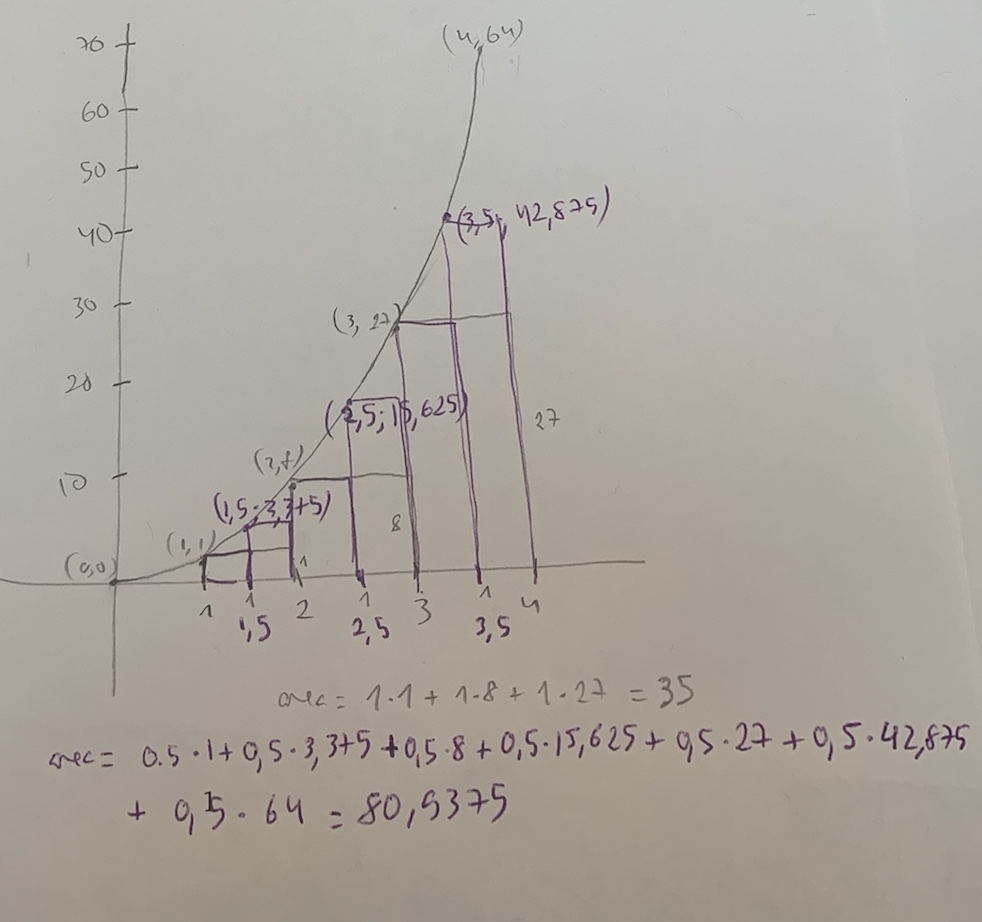
\includegraphics[scale=0.3]{pset4_rectangles.jpeg}
\item (Follow up) Now, calculate the area a second time using smaller rectangles. {\color{gray} See example above--could have selected any rectangle width. Note that we have one extra term in the example -- it should end at 3.5 and exclude the 0.5*64 for a total of approximately 53.  }
\item (Follow up) How do these areas compare? How does your finding here relate to the definition of an integral (above)?{\color{gray} The narrower the rectangle width, the closer our estimation becomes to what we'd get using an integral. Note that depending on if you do the `left' vs `right' method for rectangles (do you want to over or under-estimate the area?), your estimates may decrease (if you over estimated the area by drawing rectangles such that the right corner touches the curve) or they may increase (if you underestimated the area by drawing rectangles such that the left corner touches the curve, as seen above). In either case, we see that our estimates get closer to the true value of about 63.75 from two estimates of 35 (width=1) and 52.9 (width=0.5).}
\end{enumerate}


\item Integration Practice: Calculate the definite integrals for the following
\begin{enumerate}
\item $\int_1^4 x^3 dx${\color{gray}  =63.75}
\item $\int_0^3 x dx${\color{gray}  $=\frac{9}{2}$}
\item $\int_1^4 (6x^3-2) dx${\color{gray}  =376.5}
\item $\int_4^6 x dx${\color{gray}  =10}
\item $\int_0^y (e^x-2x^2)dx${\color{gray}  $=e^y-\frac{2y^3}{3}-1$ }
\end{enumerate}


\item Iterated Integration Practice: Calculate the  following
\begin{enumerate}
\item $\int_1^4  \int_0^2 (6x^3-2y)$ \textit{dx dy} {\color{gray} =42}
\item $\int_0^1 \int_1^x 3x-4$ \textit{dy dx} {\color{gray} =1.5}
\item $\int_0^1 \int_1^y 3x-4$ \textit{dx dy} {\color{gray} =1}
\end{enumerate}
\end{enumerate}


\end{document}




